
\documentclass{standalone}
\usepackage{tikz}
\usetikzlibrary{arrows.meta, positioning, calc, shapes.geometric}

\usepackage{amssymb} 
\usetikzlibrary{shapes.geometric}
\newcommand\ftf{0}
\begin{document}
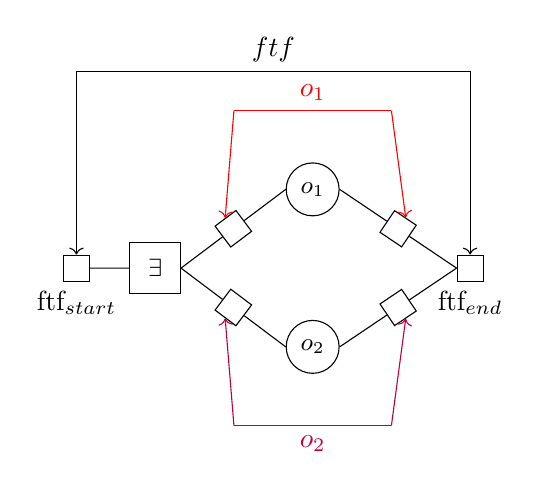
\begin{tikzpicture}[square/.style={regular polygon,regular polygon sides=4}]
    %Ftf

    \node at (\ftf, 0) [square, draw, label = below:ftf$_{start}$] (s_f) {}; 
    \node at (\ftf + 1, 0) [square, draw] (ftf) {\small $\exists$};
    \node at (\ftf + 3, 1) [circle, draw] (o5) {\small $o_1$};
    \node at (\ftf + 3, -1) [circle, draw] (o6) {\small $o_2$};
    \node at (\ftf + 5, 0) [square, draw, label = below:ftf$_{end}$] (ef) {};
  
    
    % Calculate angle between ftf and o5
    \pgfmathanglebetweenpoints{
        \pgfpointanchor{ftf}{east}
    }{
        \pgfpointanchor{o5}{west}
    }
    \edef\angleftfo5{\pgfmathresult}
  
  % Calculate angle between ftf and o5
    \pgfmathanglebetweenpoints{
        \pgfpointanchor{ftf}{east}
    }{
        \pgfpointanchor{o6}{west}
    }
    \edef\anglefo6{\pgfmathresult}
    
 % Calculate angle between ftf and o5
    \pgfmathanglebetweenpoints{
        \pgfpointanchor{o5}{east}
    }{
        \pgfpointanchor{ef}{west}
    }
    \edef\angleot5{\pgfmathresult}
     
     \pgfmathanglebetweenpoints{
        \pgfpointanchor{o6}{east}
    }{
        \pgfpointanchor{ef}{west}
    }
    \edef\angleoe5{\pgfmathresult}
    

    \node [square, draw, rotate=\angleftfo5] at ($(ftf.east)!0.5!(o5.west)$) (s1) {};
    \node [square, draw, rotate=\anglefo6] at ($(ftf.east)!0.5!(o6.west)$) (s2) {};
   
        \node [square, draw, rotate=\angleot5] at ($(o5.east)!0.5!(ef.west)$) (s1e) {};
    \node [square, draw, rotate=\angleoe5] at ($(o6.east)!0.5!(ef.west)$) (s2e) {};
   
    \draw (s_f.east) -- (ftf.west);
    
    \draw (ftf.east) -- (s1.west);
    \draw (s1.east) -- (o5.west);

    \draw (ftf.east) -- (s2.west);
    \draw (s2.east) -- (o6.west);


    \draw (o5.east) -- (s1e.west);
    \draw (s1e.east) -- (ef.west);

    \draw (o6.east) -- (s2e.west);
    \draw (s2e.east) -- (ef.west);

    \draw[->, red] (2, 2) -- (s1.north) ;
    \draw[red] (2,2) -- (4, 2) node[midway, above] {$o_1$};
    \draw[->, red] (4,2) -- (s1e.north);
        
    \draw[->, purple] (2, -2) -- (s2.south);
    \draw[purple] (2, -2) -- (4, -2) node [midway, below] {$o_2$};
    \draw[->, purple] (4,-2) -- (s2e.south);
    
    \draw[->] (0, 2.5) -- (s_f.north);
    \draw (0, 2.5) -- (5, 2.5) node [midway, above] {$ftf$};
    \draw[->] (5, 2.5) -- (ef.north);
\end{tikzpicture}
\end{document}
